\documentclass{mwart}
\usepackage{polski}
\usepackage[polish]{babel}
\usepackage{amsfonts}
\usepackage{indentfirst}
\usepackage[utf8]{inputenc}
\usepackage{amsthm}
\usepackage{multirow}
\usepackage{amsmath}
\newtheorem{tw}{Twierdzenie}
\newtheorem{df}{Definicja}
\newtheorem{zd}{Zadanie}
\newtheorem{zdt}[zd]{Zadanie*}
\title{Procesy stochastyczne\\ Zestaw zadań nr 1}
\usepackage{Sweave}
\begin{document}
\Sconcordance{concordance:Zestaw1_PS_2020.tex:Zestaw1_PS_2020.Rnw:%
1 14 1 1 0 2 1 1 6 33 1 1 3 1 2 29 1 1 7 1 5 1 2 6 1}

\maketitle

\begin{zd}
Dana jest funkcja
\begin{displaymath}
F(x) = 0\cdot\pmb{1}_{x\leq 0} + (ax^2+bx)\cdot\pmb{1}_{0<x\leq 1} + 1\cdot \pmb{1}_{x\geq 1}.
\end{displaymath}
Znajdź wszystkie pary liczb $a, b$ dla których funkcja ta jest dystrybuantą. Dla jakich wartości dystrybuanta ta jest ciągła?
\end{zd}





\begin{figure}
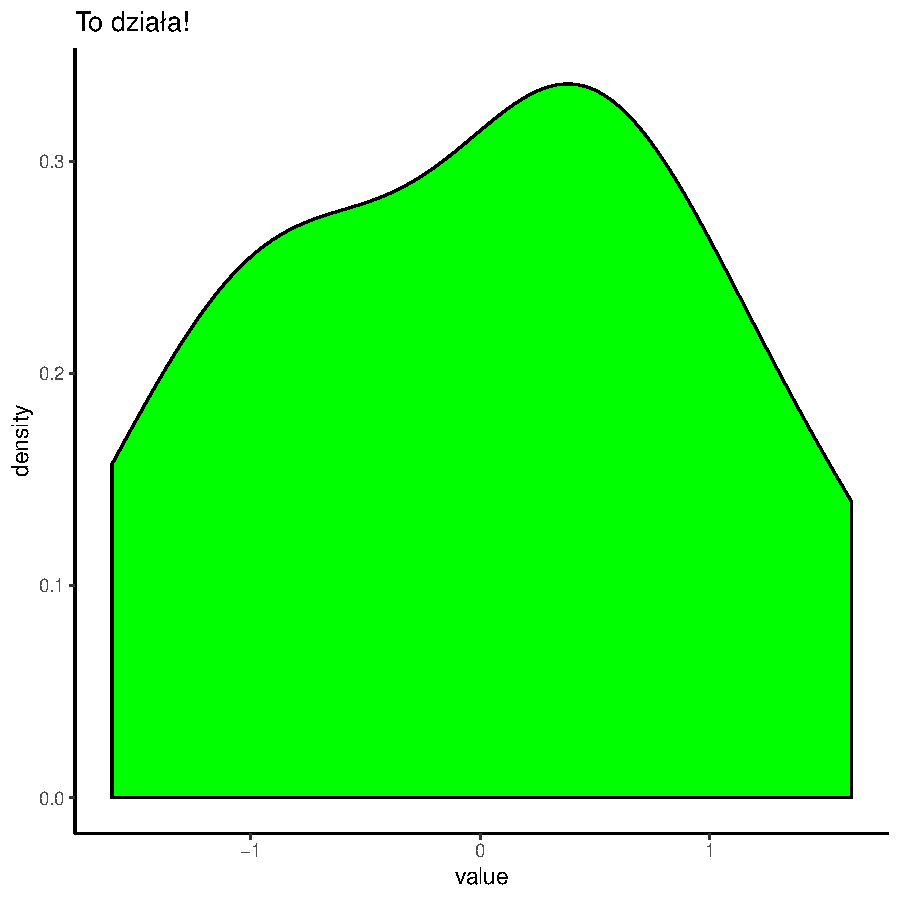
\includegraphics{Zestaw1_PS_2020-003}
\end{figure}

\end{document}
